\subsection{Electroweak Interactions}
\label{sec:Intro_Electroweak}

\begin{figure}[htb]
  \begin{center}
    {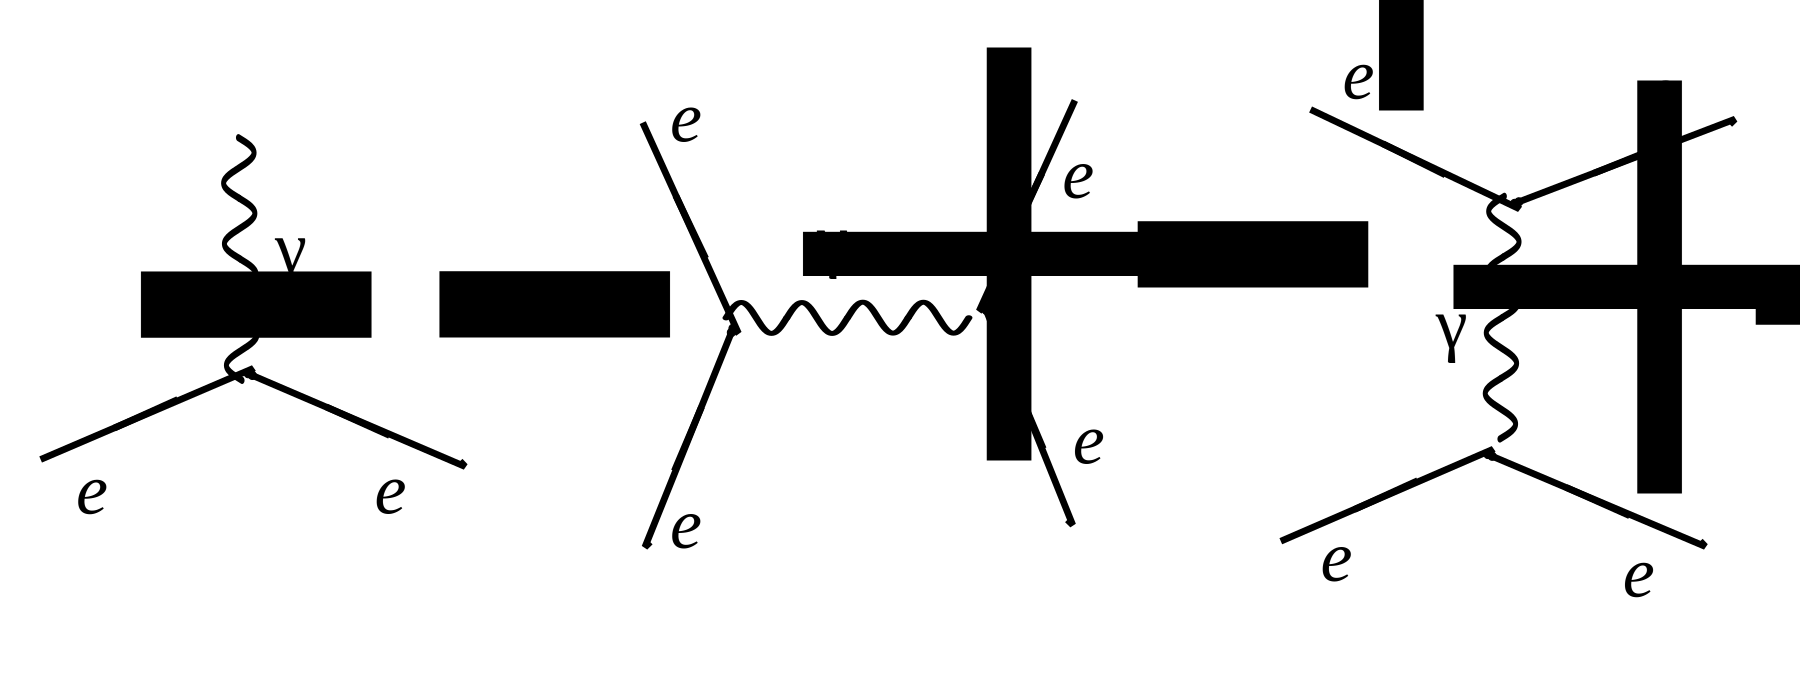
\includegraphics[width=0.90\textwidth]{../figs/Intro/feynmEM.png}}
    \caption{Electromagnetic interations}
    \label{fig:feynmEM}
  \end{center}
\end{figure}

\begin{figure}[htb]
  \begin{center}
    {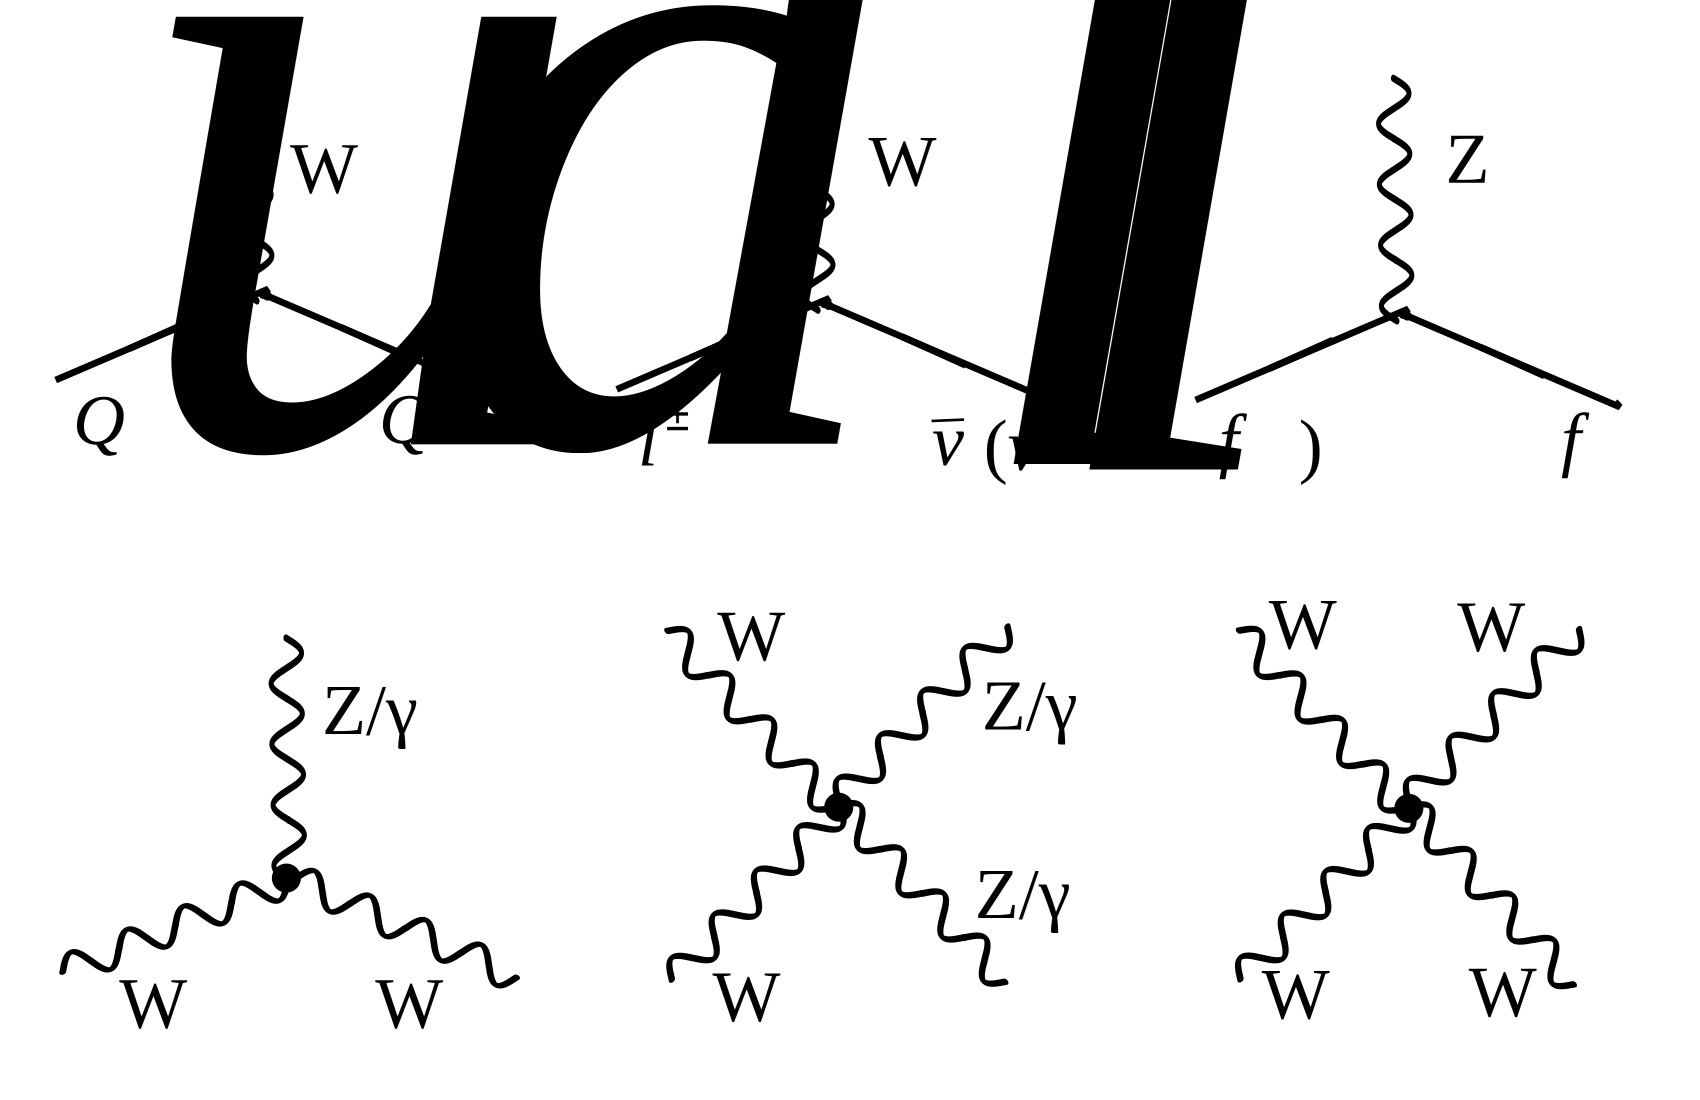
\includegraphics[width=0.90\textwidth]{../figs/Intro/feynmW.png}}
    \caption{Weak interations}
    \label{fig:feynmW}
  \end{center}
\end{figure}

% The style needs to be improved. Some places contain very chopped language.
% Consider this passage, way too “chopped”:
% > Elementary processes with W and Z bosons are shown in Fig. 3. An electric charge must be
% > conserved at any vertex. Therefore, if a charged lepton enters and radiates a W boson, a
% > neutrino or antineutrino escapes (top left in Fig. 3). That is how a W boson interacts with a
% > charged lepton and a neutrino. A lepton flavor number is always conserved in this interaction (Tab. 1).
%Consider using math mode for single character particle names, such as $c$ or $d$, to make them distinct in the text.

All electrically charged particles participate in electromagnetic interactions. Photon, the mediator of the electromagnetic interactions, is a spin-one electrically neutral massless particle. All electromagnetic interactions can be reduced to one elementary process (Fig. \ref{fig:feynmEM}, left). This process reads: an electron enters, radiates or absorbs a photon, and escapes. Although there is an electron is drawn in this figure, it can be any other charged fermion as well. Such elementary process itself is forbidden by the energy conservation law but this element is a base of actual process (for example, Fig. \ref{fig:feynmEM}, middle and right). Such graphical representations of the particle physics processes are called Feynman diagrams. 

As for the weak interactions, there are two kinds of them: neutral (mediated by a Z boson) and charged (mediated by a W boson). Elementary processes with W and Z bosons are shown in Fig. \ref{fig:feynmW}. An electric charge must be conserved at any vertex. Therefore, if a charged lepton enters and radiates a W boson, a neutrino or antineutrino escapes (top left in Fig. \ref{fig:feynmW}). That is how a W boson interacts with a charged lepton and a neutrino. A lepton flavor number is always conserved in this interaction (Tab. \ref{tab:LeptonFlavorNumber}). 

 \begin{table}[h]
  \begin{center}
  \caption{ Lepton Flavor Number}
  \begin{tabular}{|c|c|c|c|}
     particles & $L_e$ & $L_{\mu}$ & $L_{\tau}$ \\ \hline
     $e^-,\nu_e$ &  +1  &  0  &  0  \\ \hline 
     $e^+, \bar{\nu_e}$ &  -1  &  0  &  0  \\ \hline 
     $\mu^-,\nu_{\mu}$ &  0  &  +1  &  0  \\ \hline 
     $\mu^+, \bar{\nu_{\mu}}$ &  0  &  -1  &  0  \\ \hline 
     $\tau^-,\nu_{\tau}$ &  0  &  0  &  +1  \\ \hline 
     $\tau^+, \bar{\nu_{\tau}}$ &  0  &  0  &  -1  \\ \hline 
  \end{tabular}
  \label{tab:LeptonFlavorNumber}
  \end{center}
 \end{table}

From top middle diagram in Fig. \ref{fig:feynmW} we see that if a quark with Q=-1/3 enters, then a quark with Q=+2/3 escapes and, therefore, the flavor of the quarks has changed. The charged weak interaction is the only interaction which changes a quark flavor. The probability of each of three quarks with Q=+2/3 to be born is determined by the Cabibbo–Kobayashi–Maskawa matrix and is the highest for the quark of the same generation as an initial state quark (in this particular case, d is the initial state quark and u has the highest probability to be produced after an interaction with a W boson but c and t can also be produced if there is enough energy).

The right top diagram in Fig. \ref{fig:feynmW} is an emission of a Z boson off a fermion line. An electron is shown here as an example however it also could be any lepton, antilepton, quark or antiquark. All the same diagrams are possible with a photon instead of a Z boson except diagrams with neutrinos and antineutrinos.

The bottom diagrams in Fig. \ref{fig:feynmW} show self-coupling of a W boson, its interaction with Z boson and its electromagnetic radiation of a photon. WWZ, WW$\gamma$, WWZZ, WWZ$\gamma$, WW$\gamma\gamma$ and WWWW vertices are all possible in the SM.

Electromagnetic and weak interactions are unified by the electroweak theory. The mathematical formalism describing these two kinds of interactions is very similar. The difference between a photon and a Z boson is that a Z boson is massive and it can produce a neutrino-antineutrino pair or be scattered off a neutrino which a photon can not. The mass of Z boson is 91 GeV and that is why for low energies the probability of an electromagnetic process is much higher that the probability of similar neutral weak process. However, for particles with energies of E$\gg$91 GeV the mass of the Z boson can be neglected and these probabilities become the same. 
